\documentclass[12pt]{article}
\usepackage{amsmath}
\usepackage{graphicx,psfrag,epsf}
\usepackage{enumerate}
\usepackage{natbib}
\usepackage{url} % not crucial - just used below for the URL 
\usepackage[algo2e]{algorithm2e}
\usepackage{algorithmic}  
\usepackage{algorithm}
\usepackage[toc,page]{appendix}
%\pdfminorversion=4
% NOTE: To produce blinded version, replace "0" with "1" below.
\newcommand{\blind}{0}

% DON'T change margins - should be 1 inch all around.
\addtolength{\oddsidemargin}{-.5in}%
\addtolength{\evensidemargin}{-.5in}%
\addtolength{\textwidth}{1in}%
\addtolength{\textheight}{1.3in}%
\addtolength{\topmargin}{-.8in}%


\begin{document}
\def\spacingset#1{\renewcommand{\baselinestretch}%
{#1}\small\normalsize} \spacingset{1}


%%%%%%%%%%%%%%%%%%%%%%%%%%%%%%%%%%%%%%%%%%%%%%%%%%%%%%%%%%%%%%%%%%%%%%%%%%%%%%

\if0\blind
{
  \title{\bf A Continuous-time Multicast \\Network Model}
  \author{Bomin Kim\thanks{
    The authors gratefully acknowledge \textit{please remember to list all relevant funding sources in the unblinded version}}\hspace{.2cm}\\
    Department of Statistics, Pennsylvania State University,\\
  Aaron Schein\\
  College of Information and Computer Sciences, UMass Amherst,\\
    Bruce Desmarais\\
    Department of Political Science, Pennsylvania State University,\\
    and\\
    Hanna Wallach\\
    Microsoft Research NYC}
  \maketitle
} \fi

\if1\blind
{
  \bigskip
  \bigskip
  \bigskip
  \begin{center}
    {\LARGE\bf A Continuous-time Multicast Network Model}
\end{center}
  \medskip
} \fi

\bigskip
\begin{abstract}
We introduce the continuous-time multicast network model---a generative model for directed edges with multiple recipients or multiple senders. To define the model, we
integrate a dynamic version of the exponential random graph model (ERGM) and generalized linear model approach to understand who communicates with whom, and when. We use
the model to analyze emails sent between department managers in Montgomery county government in North Carolina, and international sanctions data concerning the threats and use of economic sanctions by states. Our applications demonstrate that the model is effective at predicting and explaining continuous-time networks involving edges with multiple recipients or senders.
	\end{abstract}

\noindent%
{\it Keywords:}  3 to 6 keywords, that do not appear in the title
\vfill

\newpage
\spacingset{1.45} % DON'T change the spacing!
\section{Introduction}\label{sec:intro}
\section{A Continuous-time Multicast Network Model}\label{sec:generative process}
Data generated under the model consists of $D$ unique edges. A single edge, indexed by $d \in [D]$, is represented by the three components: the sender $a_d \in [A]$, an indicator vector of recipients $\boldsymbol{r}_d = \{u_{dr} \}_{r=1}^{A}$, and the timestamp $t_d \in (0, \infty)$. For simplicity, we assume that edges are ordered by time such that $t_d \leq t_{d+1}$.
\subsection{Tie Generating Process}\label{subsec: Tie}
For every possible author--recipient pair $(a,r)_{a \neq r}$, we define the ``recipient intensity", which is the likelihood of edge $d$ being sent from $a$ to $r$:
\begin{equation}
\lambda_{adr} = {\boldsymbol{b}}^{\top}\boldsymbol{x}_{adr},
\end{equation}
where $\boldsymbol{b}$ is $P$--dimensional vector of coefficients and $\boldsymbol{x}_{adr}$ is a set of network features which vary depending on the hypotheses regarding canonical processes relevant to network theory such as popularity, reciprocity, and transitivity. In addition, we include intercept term to account for the average (or baseline) number of recipients. We place a Normal prior $\boldsymbol{b} \sim N(\boldsymbol{\mu}_b, \Sigma_b)$.

Next, we hypothesize ``If $a$ were the sender of edge $d$, who would be the recipient(s)?" To do this, we draw each sender's set of recipients from a non-empty Gibbs measure \cite{fellows2017removing}---a probability measure we defined in order to 1) allow multiple recipients or ``multicast", 2) prevent from obtaining zero recipient, and 3) ensure tractable normalizing constant. Because we allows multicast, we draw a binary (0/1) vector $\boldsymbol{u}_{ad}= (u_{ad1},
\ldots, u_{adA})$
\begin{equation} \boldsymbol{u}_{ad}  \sim
\mbox{Gibbs}(\boldsymbol{\lambda}_{ad}),
\end{equation}
where $\boldsymbol{\lambda}_{id}= \{\lambda_{adr}\}_{r=1}^A$. In particular, we define $\mbox{Gibbs}(\boldsymbol{\lambda}_{ad})$ as
\begin{equation}
\begin{aligned}
&p(\boldsymbol{u}_{ad}|\delta, \boldsymbol{\lambda}_{ad}) = \frac{\exp\Big\{\mbox{log}\big(\text{I}( \lVert \boldsymbol{u}_{ad}\rVert_1 > 0 )\big) + \sum_{r\neq a} \lambda_{adr}u_{adr}\Big\}}{Z(\boldsymbol{\lambda}_{ad})} ,
\end{aligned}
\label{eqn:Gibbs}
\end{equation}
where $Z(\boldsymbol{\lambda}_{ad})= \prod_{r \neq a} \big(\mbox{exp}(\lambda_{adr}) + 1\big)-1$ is the normalizing constant and $\lVert \cdot \rVert_1$ is the $l_1$--norm. This is equivalent to assume independent Bernoulli trial on each $u_{adr}$ with probability of 1 being logit($\lambda_{adr}$), excluding the case when all $u_{adr}=0$. We provide the derivation of the normalizing constant as a tractable form in the supplementary material. 


\subsection{Time Generating Process}\label{subsec:Time}
Similarly, we hypothesize ``If $a$ were the sender of edge $d$, when would it be sent?" and define the ``timing rate" for sender $a$
\begin{equation}
\mu_{ad} = g^{-1}(\boldsymbol{\eta}^\top \boldsymbol{y}_{ad}),
\end{equation}
where $\boldsymbol{\eta}$ is $Q$--dimensional vector of coefficients with a Normal prior $\boldsymbol{\eta} \sim N(\boldsymbol{\mu}_\eta,\Sigma_\eta)$, $\boldsymbol{y}_{ad}$ is a set of time-related covariates, e.g., any feature that could affect timestamps of the edge, and $g(\cdot)$ is the appropriate link function such as identity, log, or inverse. 

In modeling ``when", we do not directly model the timestamp $t_d$. Instead, we assume that each sender's the time-increment or ``time to next edge" (i.e., $\tau_{d} = t_d-t_{d-1}$) is drawn from a specific distribution in the exponential family.  We follow the generalized linear model framework:
\begin{equation}
\begin{aligned}
E(\tau_{ad}) &= \mu_{ad},\\
V(\tau_{ad}) &= V(\mu_{ad}),
\end{aligned}
\end{equation}
where $\tau_{ad}$ is a positive real number. Possible choices of distribution include Exponential, Weibull, Gamma, and lognormal\footnote{lognormal distribution is not exponential family but can be used via modeling of $\log(\tau_d)$.} distributions, which are commonly used in time-to-event modeling. Based on the choice of distribution, we may introduce any additional parameter (e.g., $\sigma_\tau^2$) to account for the variance. We use $f_\tau(\cdot; \mu, \sigma_\tau^2)$ and $F_\tau(\cdot; \mu, \sigma_\tau^2)$ to denote the probability density function (p.d.f) and cumulative density function (c.d.f), respectively, with mean $\mu$ and variance $\sigma^2$.

\subsection{Observed Data}\label{subsec:Observed}
Finally, we choose the sender, recipients, and timestamp---which will be observed---by selecting the sender--recipient-set pair with the smallest time-increment \cite{snijders1996stochastic}:
\begin{equation}
\begin{aligned}
a_d &= \mbox{argmin}_{a}(\tau_{ad}),\\
\boldsymbol{r}_d &= \boldsymbol{u}_{a_d d},\\
t_d &=t_{d-1} + \tau_{a_d d}.
\end{aligned}
\end{equation}
Therefore, it is a sender-driven process in that the recipients and timestamp of an edge is determined by the sender's urgency to send the edge to chosen recipients. Note that  our generative process accounts for tied events such that in case of tied events (i.e., multiple senders generated same time increments $\tau_d$), we observe all of the tied events\footnote{The order of tied events do not matter.} .
	\begin{algorithm}[H]
		\spacingset{1}
		\SetAlgoLined
		\caption{Generating Process}
		\For{d=1 to D}{
			\For{a=1 to $A$}{
				\For{r=1 to $A$}{
					\If {r $\neq$ a} {
						form $\boldsymbol{x}_{adr}$\\
						set $\lambda_{adr} = {\boldsymbol{b}}^{\top}\boldsymbol{x}_{adr}$
					}  }
					draw $\boldsymbol{u}_{ad}  \sim
					\mbox{Gibbs}(\boldsymbol{\lambda}_{ad})$\\
					form $\boldsymbol{y}_{ad}$\\
					set $\mu_{ad} = g^{-1}(\boldsymbol{\eta}^\top \boldsymbol{y}_{ad})$\\
					draw $\tau_{ad} \sim f_\tau(\mu_{ad}, \sigma_\tau^2)$
				}
				\textbf{For no tied events,}\\
				set $a_d= \mbox{argmin}_{a}(\tau_{ad})$\\
				set $\boldsymbol{r}_d = \boldsymbol{u}_{a_d d}$\\
				set $t_d =t_{d-1} + \min_a\tau_{ad}$\\\\
				\textbf{For $n$ tied events,} (i.e., $n$ senders generated same minimum time increments)\\
				set $a_d, \ldots, a_{d+n}= \mbox{argmin}_{a}(\tau_{ad})$\\
				set $\boldsymbol{r}_d=\boldsymbol{u}_{a_d d},\ldots,\boldsymbol{r}_{d+n}= ,\boldsymbol{u}_{a_{d+n} d}$\\
				set $t_d, \ldots, t_{d+n}=t_{d-1} + \min_a\tau_{ad}$\\
				jump to $d = d+n+1$
			}
			\label{alg:generative}
		\end{algorithm}
\spacingset{1.45}
\section{Posterior Inference}\label{sec:inference}
Our inference goal is to invert the generative process to obtain the posterior distribution over the unknown parameters, conditioned on the observed data and hyperparamters $(\boldsymbol{\mu}_b, \Sigma_b, \boldsymbol{\mu}_\eta, \Sigma_\eta)$. We draw the samples using Markov chain Monte Carlo (MCMC) methods, repeatedly resampling the value of each parameter from its conditional posterior given the observed data, hyperparamters, and the current values of the other parameters. We express each parameter’s conditional posterior in a closed form using the data augmentation schemes in $\boldsymbol{u}$ \cite{tanner1987calculation}. In this section, we provide each latent variable's conditional posterior. \\ \newline
First, since $u_{adr}$ is a binary random variable, new values may be sampled directly using
\begin{equation}
\begin{aligned}
&P(u_{adr}=1| \boldsymbol{u}_{ad\backslash r}, \boldsymbol{b}, \boldsymbol{x})
\propto \mbox{exp}(\lambda_{adr});\\
&P(u_{adr}=0| \boldsymbol{u}_{ad\backslash r},\boldsymbol{b}, \boldsymbol{x})\propto \text{I}(\lVert\boldsymbol{u}_{ad\backslash r}\rVert_1 > 0 ),
\end{aligned}
\label{eqn:latentreceiver}
\end{equation}
where $I(\cdot)$ is the indicator function that is used to prevent from the instances where a sender chooses zero number of recipients.\\ \newline
New values for continuous variables $\boldsymbol{b},$ and $\boldsymbol{\eta}$ and $\sigma^2_\tau$ (if applicable) cannot be sampled directly from their conditional posteriors, but may instead be obtained using the Metropolis--Hastings algorithm. With uninformative priors (i.e., $N({0},\infty)$), the conditional posterior over $\boldsymbol{b}$ is
\begin{equation}
P(\boldsymbol{b}| \boldsymbol{u}, \boldsymbol{x})\propto \prod_{d=1}^D
\prod_{a=1}^A \frac{\exp\Big\{\mbox{log}\big(\text{I}( \lVert \boldsymbol{u}_{ad}\rVert_1 > 0)\big) + \sum\limits_{r \neq a} \lambda_{adr}u_{adr}\Big\}}{Z(\boldsymbol{\lambda}_{ad})},
\end{equation}
where the two variables share the conditional posterior and thus can be jointly sampled. Likewise, assuming uninformative priors on $\boldsymbol{\eta}$ (i.e., $N({0},\infty)$) and $\sigma_{\tau}^2$ (i.e., half-Cauchy($\infty$)), the conditional posterior for no-tied event case is
\begin{equation}
P(\boldsymbol{\eta}, \sigma_\tau^2| \boldsymbol{u}, \boldsymbol{y})\propto \prod_{d=1}^D\Big(f_{\tau}(\tau_{d}; \mu_{a_d d}, \sigma_\tau^2)\times \prod_{a\neq a_d}\big(1-F_{\tau}(\tau_{d}; \mu_{a d}, \sigma_\tau^2) \big)\Big).
\end{equation}
Since we assme the existence of tied-event, the conditional posterior of $\boldsymbol{\eta}$ and $\sigma_{\tau}^2$ should be written as
\begin{equation}
P(\boldsymbol{\eta}, \sigma_\tau^2| \boldsymbol{u}, \boldsymbol{y})\propto \prod_{m=1}^M\Big(\prod_{d:t_d=t_m^*}f_{\tau}(t_m^*-t_{m-1}^*; \mu_{a_d d}, \sigma_\tau^2)\times \prod_{a \notin \{a_d\}_{d:t_d=t_m^*}}\big(1-F_{\tau}(t_m^*-t_{m-1}^*; \mu_{a d}, \sigma_\tau^2) \big)\Big),
\end{equation}
where $t_1^*,\ldots,t_M^*$ are the unique timepoints across $D$ events ($M \leq D$). If $M=D$ (i.e., no tied events), Equation (10) reduces to Equation (9).

 \begin{algorithm}[H]
 			\spacingset{1}
 	\SetAlgoLined
 	\caption{MCMC Algorithm}
 	set initial values of $\boldsymbol{b}, \boldsymbol{\eta}, \sigma_\tau^2$\\
 	\For{o=1 to outer}{
 	 		\For{d=1 to D}{
 			\For{a = 1 to A}{
 				\For{r = a to A}{
 					\If {r $\neq$ a} {
 						update $u_{adr}$ using Gibbs update --- Equation (7)
 					}
	 			}
 			}
 		}
 		 		\For{n=1 to inner1}{
 		 			update $\boldsymbol{b}$ using Metropolis-Hastings --- Equation (8)
 				}
 		\For{n=1 to inner2}{
 				update $\boldsymbol{\eta}$ and $\sigma_\tau^2$ using Metropolis-Hastings --- Equation (10)
 		}
 			\For{n=1 to inner3}{
 				update $\sigma_\tau^2$ using Metropolis-Hastings --- Equation (10)
 			}
 }
 	Summarize the results with: \\last chain of $\boldsymbol{b}$, and last chain of $\boldsymbol{\eta}$ and $\sigma_\tau^2$ 
 \end{algorithm}
 
 \section{Getting It Right}\label{sec:GiR}
 \begin{figure}[H]
 	\centering
 	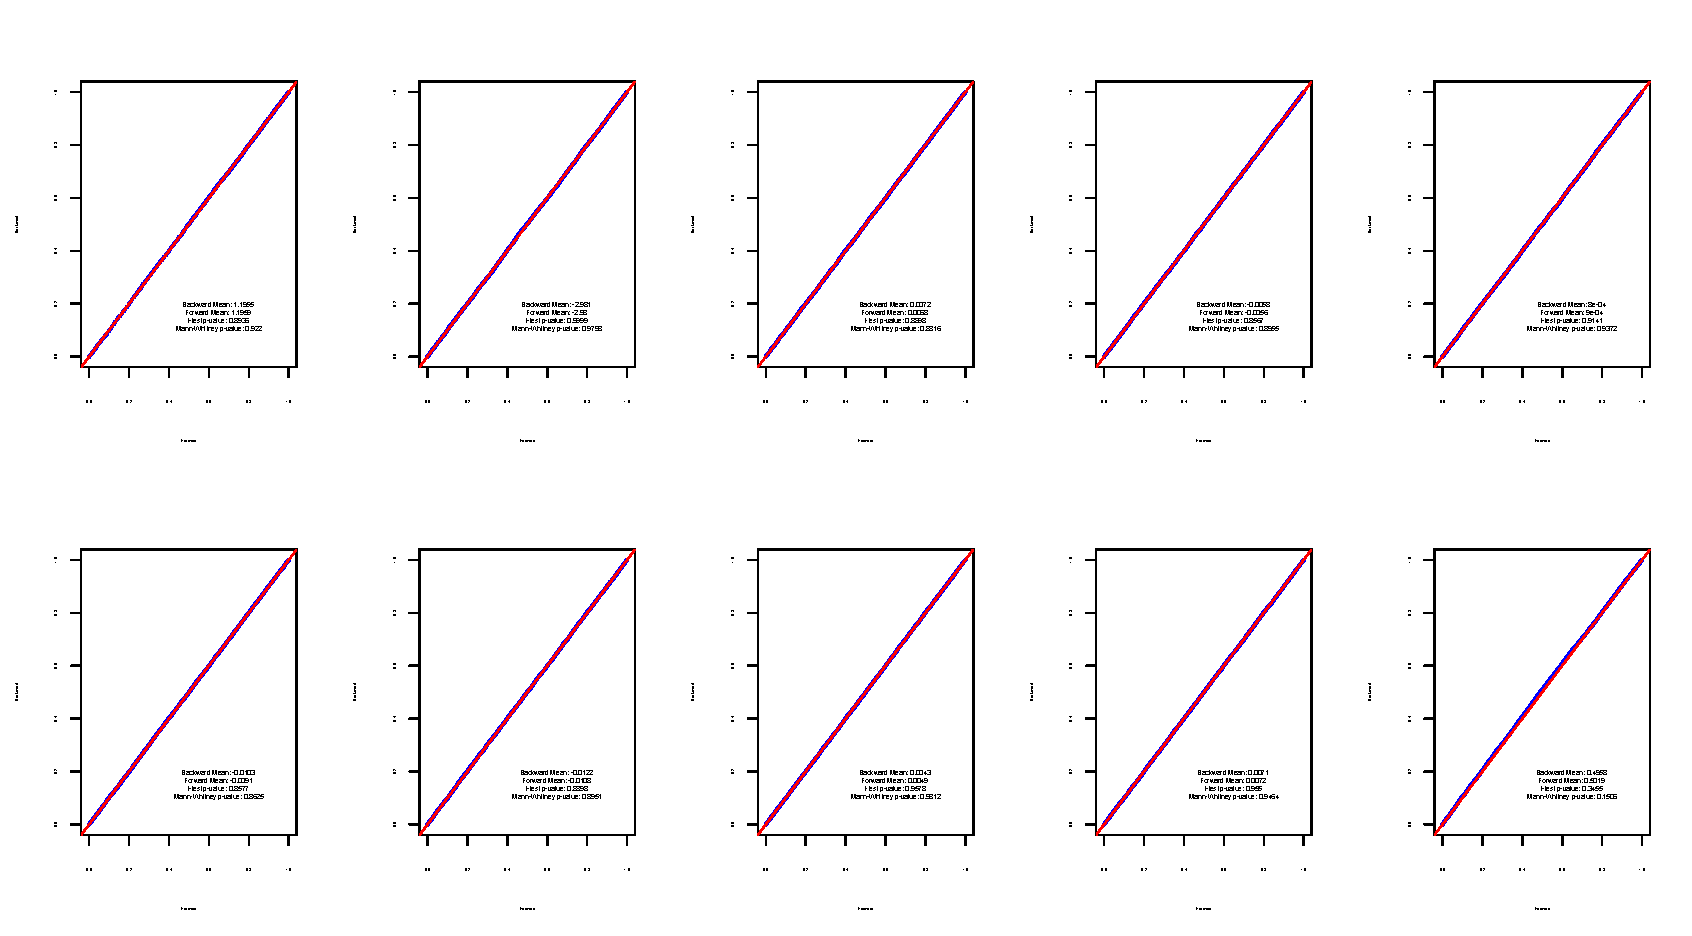
\includegraphics[width=1\textwidth, trim = 0.5cm 1cm 0.5cm 1cm, clip=true]{Multicast_Schein.pdf}	
 	\caption {Schein test results when we run 5 outer iterations and 5 inner iterations using 20,000 samples (with $D = 100, A = 5, P = 5, Q = 3$)}
 	\label{figure:GiR}
 \end{figure}
 
\section{Case Studies}\label{sec:case studies}
We now present two case studies applying our method to 1) county government emails (single sender multiple recipients) and 2) international sanctions (multiple senders single recipient). For each case study,
we formulate the network statistics $\boldsymbol{x}$ and timestamp statistics $\boldsymbol{y}$ and ground them in
illustrative examples. We then report a suite of experiments that test our method’s ability to form the posterior distribution over latent variables for different types of data. 
 	   \subsection{Case Study 1: County Government Emails}\label{subsec:Emails}
 	  	   \subsubsection{Montgomary County Data}\label{subsubsec:Montgomery}
 	   Our data come from the North Carolina county government email dataset collected by \cite{ben2017transparency} that includes internal email corpora covering the inboxes and outboxes of managerial-level employees of North Carolina county governments. Out of over twenty counties, we chose Montgomery County to 1) test our model using data with a lot of multicast edges (16.76\%), and 2) limit the scope of this initial application. The Montgomery County email network contains 680 emails, sent and received by 18 department managers over a period of 3 months (March--May) in 2012. 
 	   \subsubsection{Covariates}\label{subsec:Covariates_email}
In the example of email networks, we form the covariate vector $\boldsymbol{x}_{adr}$ using time-varying network statistics based on the time interval prior to and including $t_{d-1}$. Along with intercept term, we compute eight network statistics \cite{PerryWolfe2012}, where the time interval tracks 7 days prior to the last email was sent $l_d = (t_{d-1}-7\mbox{days}, t_{d-1}]$. 
\begin{itemize}
	 			\spacingset{1}
	\item[1.] intercept $\boldsymbol{x}_{adr1} =1$;
	\item[2.] outdegree $\boldsymbol{x}_{adr2} =\sum\limits_{d^\prime: t_{d^\prime} \in l_d} I(a_{d^\prime} = a)$;
	\item[3.] indegree $\boldsymbol{x}_{adr3}=\sum\limits_{d^\prime: t_{d^\prime} \in l_d} I(u_{d^\prime r} = 1)$;
	\item[4.] send $\boldsymbol{x}_{adr4}=\sum\limits_{d^\prime: t_{d^\prime} \in l_d} I(a_{d^\prime} = a)I(u_{d^\prime r} = 1)$;
	\item[5.] receive $\boldsymbol{x}_{adr5}=\mbox{send}(r,a)$;
	\item[6.] 2-send $\boldsymbol{x}_{adr6} = \sum\limits_{h \neq a, r} \mbox{send}(a,h)\mbox{send}(h,r)$;
	\item[7.] 2-receive $\boldsymbol{x}_{adr7}= \sum\limits_{h \neq a, r} \mbox{send}(h,a)\mbox{send}(r,h)$;
	\item[8.] sibling $\boldsymbol{x}_{adr8}=\sum\limits_{h \neq a, r} \mbox{send}(h,a)\mbox{send}(h,r)$;
	\item[9.] cosibling $\boldsymbol{x}_{adr9}=\sum\limits_{h \neq a, r} \mbox{send}(a,h)\mbox{send}(r,h)$;
\end{itemize}
where $I(\cdot)$ is an indicator function.\\ \newline
For time-related covariates $\boldsymbol{y}_{ad}$ in Section \ref{subsec:Time}, we form the covariate vector $\boldsymbol{y}_{ad}$ using the seven statistics which may possibly effect ``time to send the next document". Note that these statistics could depend on $a$ only, $d$ (or $t_d$) only, or both $a$ and $d$. Specifically, the statistics are
\begin{itemize}
	\spacingset{1}
	\item[1.] intercept $\boldsymbol{y}_{ad1} =1$;
	\item[2.] outdegree $\boldsymbol{y}_{ad2} =\sum\limits_{d^\prime: t_{d^\prime} \in l_d} I(a_{d^\prime} = a)$;
	\item[3.] indegree $\boldsymbol{y}_{ad3}=\sum\limits_{d^\prime: t_{d^\prime} \in l_d} I(u_{d^\prime a} = 1)$;
	\item[4.] gender $\boldsymbol{y}_{ad4}=I(a= \mbox{female})$;
	\item[5.] manager $\boldsymbol{y}_{ad5}=I(a= \mbox{County Manager})$;
	\item[6.] weekend $\boldsymbol{y}_{ad6} = I(t_{d-1}= \mbox{weekend})$;
	\item[7.] am/pm $\boldsymbol{y}_{ad7}= I(t_{d-1}= \mbox{pm})$;
\end{itemize}
\subsubsection{Parameter Estimation and Interpretation}\label{subsubsec:Result_email}
\subsection{Case Study 2: International Sanctions}\label{subsec:International Sanctions}
\subsubsection{Threat and Imposition of Sanctions (TIES) Data}\label{subsubsec:TIES}
We processed the threat and imposition of sanctions (TIES) data \citep{morgan2014threat} that includes the records of international sanctions---defined as actions that one or more countries take to limit or end their economic relations with a target country in an effort to persuade that country to change one or more of its policies---from 1945 to 2005.
\subsubsection{Covariates}\label{subsec:Covariates_sanction}
\subsubsection{Parameter Estimation and Interpretation}\label{subsubsec:Result_sanction}

\subsection{Experiment}\label{subsubsec:Experiment_email}
We evaluate the model's ability to predict ties from the Montgomery County email network and the threat and imposition of sanctions (TIES) data, conditioned on their ``training" part of the data. We separately formed a test split of each three components---author, recipients, and timestamps---by randomly selecting ``test" data with probability $p=0.1$. Any missing variables were imputed by drawing samples from their conditional posterior distributions, given the observed data, estimates of latent variables, and current estimates of test data. The full conditional posterior distributions for ``test" author, recipients, and timestamps are provided in the supplementary material. We then run inference to update the latent variables given the imputed and observed data. We iterate the two steps---imputation and inference---multiple times to obtain enough number of estimates for ``test" data. Algorithm \ref{alg:PPE} outlines this procedure.

\begin{algorithm}[H]
	\spacingset{1}
	\caption{Out-of-Sample Tie Predictions}
	\label{alg:PPE}
	\begin{algorithmic}
		\STATE {\bfseries Input:} data $ \{ (a_d, \boldsymbol{r}_d, t_d)\}_{d=1}^D$, \\
		number of new data to generate $R$,\\
		hyperparameters $(\boldsymbol{\mu}_b, \Sigma_b, \boldsymbol{\mu}_\eta, \Sigma_\eta)$\\
		\vskip 0.1in
		\textbf{Test splits:}	
		\STATE Draw test authors with $p=0.1$ (out of $D$ authors) 
		\STATE Draw test elements of recipient vector 
		with $p=0.1$ (out of $D\times (A-1)$ receipient indicators $\{\{\boldsymbol{r}_{dr}\}_{r\in [A]_{\backslash a_d}}\}_{d=1}^D$)
		\STATE Draw test timestamps with $p=0.1$  (out of $D$ timestamps) 
		\STATE Set the ``test" data as ``missing" (NA)
		\vskip 0.1in
		\textbf{Imputation and inference:}	
		\STATE Initialize the parameters $(\boldsymbol{b}, \boldsymbol{\eta}, \boldsymbol{u}, \sigma^2_\tau)$
		\FOR{$r=1$ {\bfseries to}  $R$}
		\FOR{$d=1$ {\bfseries to}  $D$}
		\IF{$a_d=$  NA}
		\FOR{$a=1$ {\bfseries to} $A$}
		\STATE Compute $\pi_{a} $ using $P(a_d= a | \cdot)$
		\ENDFOR
		\STATE Draw $a_d \sim \mbox{Multinomial}(\pi)$
		\ENDIF
		\FOR{$r\in [A]_{\backslash a_d}$}
		\IF{$r_{dr}=$ NA}
		\STATE Draw $r_{dr}$ using $P(r_{dr}= 1 | \cdot)$ and $P(r_{dr}= 0| \cdot)$ 
		\ENDIF
		\ENDFOR
		\IF{$t_d=$ NA}
		\STATE Draw proposal $\boldsymbol{\tau}^{new}_d \sim f_\tau(\mu_{a_dd}, \sigma^2_\tau)$
		\STATE Use Metropolis-Hastings to decide accept or reject using the probability
		\begin{equation*}
		\footnotesize
		\frac{P(\boldsymbol{\tau}^{new}_d|\mu_{a_dd}, \sigma^2_\tau) P(\boldsymbol{\tau}^{new}_d| \cdot)}{P(\boldsymbol{\tau}^{old}_d|\mu_{a_dd}, \sigma^2_\tau) P(\boldsymbol{\tau}^{old}_d| \cdot)},
		\end{equation*}
		where $\boldsymbol{\tau}^{old}_d$ is from earlier iteration.
		\ENDIF
		\STATE Run inference and update $(\boldsymbol{b}, \boldsymbol{\eta},\boldsymbol{u}, \sigma^2_\tau)$ given the imputed and observed data
		\ENDFOR
		\STATE Store the estimates for ``test" data
		\ENDFOR
	\end{algorithmic}
\end{algorithm}
NOTE: we assume independent Bernoulli trial on $u_{adr}$. Then, does it matter to have test `elements' for the recipient vector instead of having the test `recipient vectors'?

\subsection{Posterior Predictive Checks}\label{subsubsec:PPC_email} 	   
Finally, we perform posterior predictive checks \cite{rubin1984bayesianly} to evaluate the appropriateness of our model specification for the Montgomery County email data and the threat and imposition of sanctions (TIES) data. We formally generated entirely new data, by simulating ties and timestamps $\{(a_{d}, \boldsymbol{r}_{d}, t_{d})\}_{d=1}^D$ from the genenerative process in Section \ref{sec:generative process}, conditional upon a set of inferred parameter values from the inference in Section \ref{sec:inference}. For the test of goodness-of-fit in terms of network dynamics, we use multiple network statistics that summarize meaningful aspects of the Montgomery County email data and the threat and imposition of sanctions (TIES) data: indegree distribution, outdegree distribution, recipient size distribution, time-increments distribution, the edgewise shared partner distribution, and the geodesic distance distribution. We then generated 500 synthetic networks from the posterior predictive distribution.
\begin{algorithm}[H]
	\spacingset{1}
	\caption{Generate new data for PPC}
	\begin{algorithmic}
		\STATE \textbf{Input}: number of new data to generate $R$,\\
		estimated latent variables $(\boldsymbol{u}, \boldsymbol{b}, \boldsymbol{\eta},  \sigma_\tau^2)$\\
		\vskip 0.1in
		
		\FOR{$r=1$ {\bfseries to}  $R$}
		\FOR{$d = 1$ {\bfseries to}  $D$} 
		\STATE  Compute $\boldsymbol{x}_{d}$ and $\boldsymbol{y}_{d}$ given $\{(a_{d}, \boldsymbol{r}_{d}, t_{d})\}_{[1:(d-1)]}$
		\STATE	Draw ($a_{d}$, $\boldsymbol{r}_{d}$, $t_{d}$) following Section \ref{sec:generative process}\\
		\ENDFOR
		\STATE Store every $r^{th}$ new data $\{(a_{d}, \boldsymbol{r}_{d}, t_{d})\}_{d=1}^D$ 
		\ENDFOR
	\end{algorithmic}
\end{algorithm}       

\section{Conclusion}\label{sec:conclusion}
\newpage
\bibliographystyle{agsm}
\bibliography{multicastnetwork}
\begin{appendices}
\section{Normalizing constant of Gibbs measure}\label{sec: non-empty Gibbs measure}
The non-empty Gibbs measure \cite{fellows2017removing} defines the probability of author $a$ selecting the binary recipient vector $\boldsymbol{u}_{ad}$ as
\begin{equation*} 
\begin{aligned}
& P(\boldsymbol{u}_{ad}|\boldsymbol{\lambda}_{ad} ) = \frac{\exp\Big\{ \mbox{log}\big(\text{I}(\lVert \boldsymbol{u}_{ad} \rVert_1 > 0)\big) + \sum_{r \neq a} \lambda_{adr}u_{adr} \Big\}}{Z(\boldsymbol{\lambda}_{ad})}.
\end{aligned}
\end{equation*}

To use this distribution efficiently, we derive a closed-form expression for $Z(\boldsymbol{\lambda}_{id})$ that does not require brute-force summation over the support of $\boldsymbol{u}_{ad}$ (\textit{i.e.} $\forall \boldsymbol{u}_{ad} \in [0,1]^A$). We recognize that if $\boldsymbol{u}_{ad}$ were drawn via independent Bernoulli distributions in which $P({u}_{adr}=1|\delta, \boldsymbol{\lambda}_{ad})$ was given by logit$(\lambda_{adr})$, then 
\begin{equation*}
P(\boldsymbol{u}_{ad}|\boldsymbol{\lambda}_{ad}) \propto \exp\Big\{\sum_{r \neq a } \lambda_{adr}u_{adr}\Big\}.  	 
\end{equation*}
This is straightforward to verify by looking at 
\begin{equation*}
\begin{aligned}
&P(u_{adr}=1|\boldsymbol{u}_{ad[-r]}, \boldsymbol{\lambda}_{ad})
=\frac{ \exp{(\lambda_{adr})}}{\exp{(\lambda_{adr})} + 1}.\end{aligned}\end{equation*}
We denote the logistic-Bernoulli normalizing constant as $Z^{l}(\boldsymbol{\lambda}_{ad})$, which is defined as 
\begin{equation*}
Z^{l}(\delta,\boldsymbol{\lambda}_{ad})=\sum_{\boldsymbol{u}_{ad} \in [0,1]^{A}} \exp\Big\{\sum_{r\neq a} \lambda_{adr}u_{adr}\Big\}.
\end{equation*}
Now, since 
\begin{equation*}
\begin{aligned}
&\exp\Big\{ \mbox{log}\Big(\text{I}(\lVert \boldsymbol{u}_{ad} \rVert_1 > 0)\Big) + \sum_{r \neq a} \lambda_{adr}u_{adr} \Big\}\\&= \exp\Big\{  \sum_{r \neq a} \lambda_{adr}u_{adr} \Big\},
\end{aligned}
\end{equation*}
except when $\lVert \boldsymbol{u}_{ad} \rVert_1=0$, we note that 
\begin{equation*}
\begin{aligned}
Z(\boldsymbol{\lambda}_{ad})& = Z^{l}(\boldsymbol{\lambda}_{ad}) -\exp\Big\{ \sum\limits_{\forall u_{adr}=0}\lambda_{adr}u_{adr} \Big\}
\\& = Z^{l}(\lambda_{a}^{(d)}) -  1.
\end{aligned}
\end{equation*}
We can therefore derive a closed form expression for $Z(\delta,\boldsymbol{\lambda}_{ad})$ via a closed form expression for $Z^{l}(\delta,\boldsymbol{\lambda}_{ad})$. This can be done by looking at the probability of the zero vector under the logistic-Bernoulli model:
\begin{equation*}
\begin{aligned}
&\frac{\exp\Big\{ \sum\limits_{\forall u_{adr}=0}\lambda_{adr}u_{adr} \Big\}}{Z^{l}(\boldsymbol{\lambda}_{ad})}= \prod_{r \neq a}   \Big(1-\frac{ \exp{(\lambda_{adr})}}{\exp{(\lambda_{adr})} + 1}\Big).
\end{aligned}  
\end{equation*}
Then, we have 
\begin{equation*}
\begin{aligned}
& \frac{1}{Z^{l}(\boldsymbol{\lambda}_{ad})} &= \prod\limits_{r \neq a}\frac{1}{ \exp(\lambda_{adr})+ 1}.
\end{aligned}  
\end{equation*}
Finally, the closed form expression for the normalizing constant under the non-empty Gibbs measure is  \begin{equation*}
\begin{aligned}Z(\boldsymbol{\lambda}_{ad}) = \prod_{r \neq a } \big(\mbox{exp}(\lambda_{adr}) + 1\big)-1.
\end{aligned}  
\end{equation*}
 
	\end{appendices}
\end{document}